\documentclass[10pt,conference,compsocconf]{IEEEtran}

\usepackage{hyperref}
\usepackage{graphicx}	% For figure environment

% Packages added by Joachim

%drow graph
\usepackage{fancybox}
\usepackage{tikz}
\usepackage{capt-of}
\usepackage{verbatim}

% cancel math expression
\usepackage{cancel}


\begin{document}
\title{PCML CS-433: Higgs Challenge Project}

\author{
  Joachim Muth, SCIPER 214757, joachim.muth@epfl.ch\\
  Junze Bao, SCIPER 266983, junze.bao@epfl.ch\\
  Chanhee Hwang, SCIPER 260872, chanhee.hwang@epfl.ch\\ \\
  \textit{School of Computer and Communication Sciences, EPF Lausanne, Switzerland}
}

\maketitle

%========================
\begin{abstract}
...
\end{abstract}

%========================
\section{Introduction}
The ATLAS experiment consists of collisions between protons. Particles created by these collisions are detected by sensors, producing a sparse vector of about a hundred thousand dimensions. Analyzing these data, ATLAS team try to estimate if the detected particles comes from a Higgs boson decay.

The \emph{Higgs boson machine learning challenge} consists of a large dataset of particles decay detections labeled as Higgs or background. The dataset is composed of thirty features and is already cleaned from a lot of well-known background effect well-known by the ATLAS team. Also, in order to balance the great number of background events compared to Higgs events, the size of both dataset is balanced.~\cite{higgsChallenge}

%========================
\section{Models and Methods}

\subsection{Splitting the data}
In order to chose which features to keep in the machine learning modelling we did, and to deal with the great number of \emph{NaN} in the data set, we analyzed their distrubution. 

It show that it's possible to cathegorize the events into four different sets based on the number of jets (\emph{int} $\in [0, 3]$). There is a physics reason behind it, since some measures make no sens for some jet numbers. \cite{higgsChallenge}.

Once this split proceeded, subsets share all the same defined features, except the estimated mass $m_H$ of the Higgs boson candidate. Once again, these subsets are split into two subsets to obtain, finally, eight different subsets to model (see figure \ref{split})

\begin{figure}[tbph] %-------TIKZ PICTURE---------
  \centering
  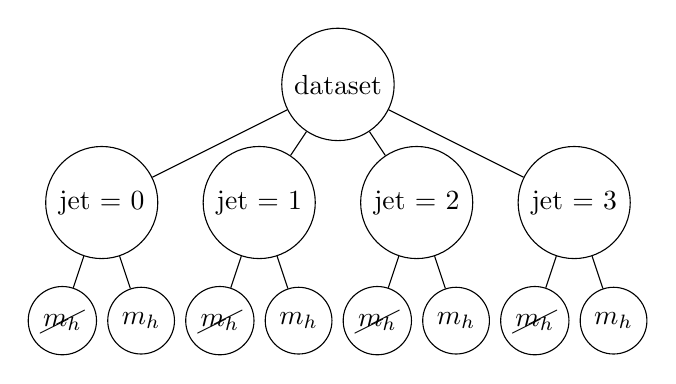
\begin{tikzpicture}[level/.style={sibling distance=20mm/#1}]
  \node [circle,draw] (z){dataset}
  child {node [circle,draw] (a) {jet = 0}
    	child {node [circle,draw] (b) {$\cancel{m_h}$}
    	}
  	child {node [circle,draw] (g) {$m_h$}
  	}
  }
  child {node [circle,draw] (j) {jet = 1}
      	child {node [circle,draw] (b) {$\cancel{m_h}$}
    	}
    	child {node [circle,draw] (g) {$m_h$}
    	}
  }
    child {node [circle,draw] (j) {jet = 2}
        child {node [circle,draw] (b) {$\cancel{m_h}$}
    	}
    	child {node [circle,draw] (g) {$m_h$}
    	}
  }
    child {node [circle,draw] (j) {jet = 3}
        child {node [circle,draw] (b) {$\cancel{m_h}$}
    	}
    	child {node [circle,draw] (g) {$m_h$}
    	}
  };
  \end{tikzpicture}
  \caption{Split of the dataset into eight different cathegories}
  \vspace{-3mm}
  \label{split}
\end{figure}




%========================
\section{Results}



%========================
\section{Discussion}


%========================
\section{Summary}

...


\bibliographystyle{IEEEtran}
\bibliography{literature}

\end{document}
